\subsection*
{\href{http://cst.mi.fu-berlin.de/intern/19606-P-MPP/Aufgaben/040203.html}
{Aufgabe 7: Dynamische Taktfrequenzumschaltung}}

\subsubsection*{Quelltext}

\lstinputlisting[linerange=10-21,firstnumber=10,caption=aufgabe07.c]
{../MPP_WS1011/aufgaben/aufgabe07.c}

Diese Macros erlauben das schnelle Zurücksetzen der jeweiligen Bitgruppen der DCOCTL, BCSCTL1 und BCSCTL2 Register auf 0.

\begin{lstlisting}[caption=Macros]
#define RSEL_RESET      (BCSCTL1 &= ~(RSEL0 | RSEL1 | RSEL2))
#define DCO_RESET       (DCOCTL  &= ~(DCO0 | DCO1 | DCO2))
#define MOD_RESET       (DCOCTL  &= ~(MOD0 | MOD1 | MOD2 | MOD3 | MOD4))
#define DIVM_RESET      (BCSCTL2 &= ~(DIVM0 | DIVM1))
\end{lstlisting}

Die Interruptroutine für einen Tastendruck, stellt unter Zuhilfenahme obiger Macros und durch Setzen entsprechender Werte in den Clock-Kontrollregistern einen der beiden Frequenzpunkte ein. Eine Variable $freqState$ speichert, ob der Controller mit hohem oder niedrigem Takt bestrieben wird.

\lstinputlisting[linerange=57-95,firstnumber=57,caption=interrupts\_a07.c]
{../MPP_WS1011/aufgaben/interrupts_a07.c}

\subsubsection*{Messwerte}

Je höher die Frequenz, desto höher der Stromverbrauch:

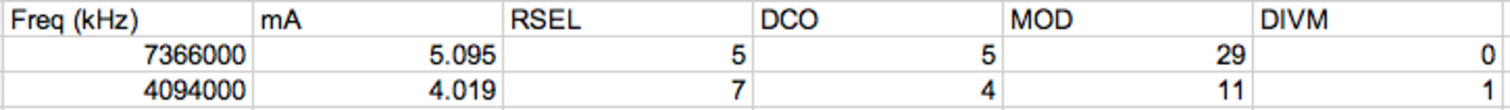
\includegraphics[width=\textwidth]{aufgaben/07/CLK.pdf}
